\subsubsection{The Launcher}
\textit{Note that the Launcher was not implemented as part of the thesis.}
The Launcher should show up when the application is launched and in many ways function as a "server browser".
Here the user can decide between hosting a session on a 3D model he or she has access to, or join an existing session from a list/browser.
When the user wishes to initiate or join a session with a particular 3D model to be inspected, he/she should be able to:

\paragraph{When hosting}a session, the user should be able to:
\begin{itemize}
	\item Specify a 3D model from a standard file format to host the session on.
	\item Give the session a name
	\item Define a password, which will be required to enter the session. 
	\item Choose between different visibility settings for the session (e.g~whether it should show up in the session list)
\end{itemize}

\paragraph{When joining}a session, the user  should be able to:
\begin{itemize}
	\item Choose a session from the session list and click the join-button to enter.
	\item Enter the name of a session in the search text field to search for a session by name.
			This should also enable to find sessions that are otherwise "hidden".
\end{itemize}	

% Mockup for the launcher?

\subsubsection{The Inspector}
Once a user has either created or joined a session and is loaded into the model, he or she should be able to do the following:

\paragraph{Choose between Virtual Reality Mode and Desktop Mode.} Virtual reality mode is meant to be used with a virtual reality headset
and sets up the correct settings (e.g the field of view). Desktop mode is meant to be used without a virtual reality headset and instead used
a regular display. This modes sets up the best setting for regular display usage, and if a virtual reality headset is attached the input from it will be ignored 
(e.g.~To avoid its orientation affecting the camera in the application).

\paragraph{Look around.} By looking around the camera should rotate to the desired direction, but the player model should keep its orientation 
(e.g.~"forward" is the same directing independent of where the user is looking). Looking around can only be achieved by the user turning his or her 
head while wearing a virtual reality HMD and having the application run in VR mode.

\paragraph{Rotate (i.e change orientation).} When rotating the camera and the player model should rotate in the desired direction (e.g.~"forward" is where the player model is
facing after the rotation).
Rotation should allow pitching and yawing (rotation along the Y and Z axis), but not rolling (rotation along the X axis) as this might cause the user discomfort, especially when
using a virtual reality headset, and has little to no practical implication. See \ref{the_six_degrees_of_freedom} for an illustration of this. 
Rotation should be possible either by using a gesture or by moving the mouse.

\paragraph{Move (i.e change position).} The user should be able to move freely along the X, Y and Z axis, thus moving both in the horizontal and vertical plane. 
This movement should happen without regard for any external forces, such as gravity or collision. The user should be able to this movement by using the keyboard or 
by using gestures. On the keyboard six different keys should be used (forward, backwards, left, right, up and down), while the same should be accomplished by
either three distinct gestures (forward/backward, left/right, up/down) or one combined gesture (forward/backwards/left/right/up/down).

\begin{figure}%[h!] %[H]
	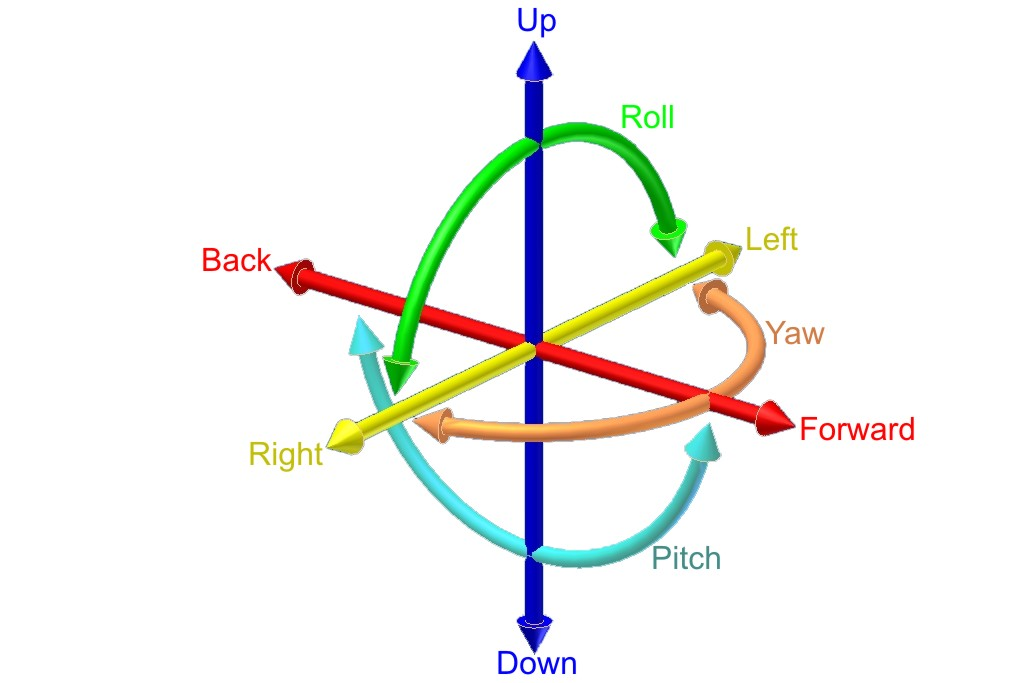
\includegraphics[width=\linewidth]{pictures/the_six_degrees_of_freedom.jpg}
	\caption[The six degrees of freedom]{The six degrees of movement in a three-dimensional space. A rigid body in this space can change \textbf{position} along the X axis (left/right), 
	Y axis (up/down)and Z axis (forward/backward), or change \textbf{rotation/orientation} along the X axis (rolling), Y axis (pitching) and Z axis (yawing).
	Picture from \citet{6DOF}}
	\label{fig:the_six_degrees_of_freedom}
\end{figure} 

\paragraph{Annotate a point.} The user should be able to create and attach an annotation, i.e a unit of information related to an aspect of the 3D model, to a point on a surface in
the 3D model. These annotations can visually be represented as a sphere or orb in the model (to make it uniformly visible from all angles). This should be accomplished by
either clicking the mouse or using a gesture. 

\paragraph{Annotate an object.} The user should be able to annotate a whole object in the 3D model, as opposed to only annotating a point on it. When an object, such
as a wall, pipe or gear, is annotated in this fashion it should be highlighted or marked in some distinct manner. This should be accomplished by
either clicking the mouse or using a gesture. 

\paragraph{Edit an annotation.} The user should be able edit an annotation, either tied to a point or an object, by clicking on the annotation. 
This should bring up a form, that should at least offer the following functionality:
\begin{itemize}
	\item Textual input through a text box.
	\item A submit-button to save the current annotation state and close the annotation form.
	\item A cancel-button to close the annotation form without saving any changes.
	\item A delete-button to delete the annotation, i.e removing the annotation sphere or highlighting and all it's associated information. 
	\item Choosing between several annotation categories, labels or states by clicking on one of several associated buttons. 
			These should function as radio-buttons, i.e when one is selected the others are always deselected.
			These categories could refer to the progress status of the task the annotation represents, e.g.~"unresolved", "work in progress" and "approved",
			or they could represent the nature of the annotation itself, e.g.~ "information", "warning" and "error".

	\item A virtual keyboard that can be used instead of the physical keyboard to input text. This is primarily included so the user can input text using 
			gesture recognition technology.
\end{itemize}

\paragraph{Access a menu.} The user should be able to access a menu that offers different options related to the usage of the application.
The menu should allow the the user to:
\begin{itemize}
	\item Go back to the origin position, e.g move and rotate the player model to the same position and orientation as when the application was started.
	\item Choose whether the annotation spheres should be globally visible (e.g.~visible through walls), only visible with line-of-sight or invisible.
		  The first of these options is there to ensure that the user easily can see every annotation, regardless of where the user is in the model,
		  while the other options are there for preference. The default should be global visibility.
	\item Toggle between (i.e turn off or turn on) gesture recognition based on whether it's already turn on or off.
		  This is to enable the user to use his or her hands without it having effect on the application. 
	\item Toggle between having X, Y, and Z axis movement as three separate gestures (forward/backward, left/right, up/down) or one (forward/backwards/left/right/up/down). 
\end{itemize}


Actions done during the 3D model session (such as annotating an object) should continuously be stored in a database. 
If a user wants to re-enter the session at a later time, this database is read, and the actions done in previous sessions are loaded into the model.
By utilizing a database 
in this way the model files themselves can also remain unedited throughout a session, as opposed to saving annotations into the model files itself, 
which could be more inefficient and create model versioning issues. 
Another upside with utilizing a database is that it enables exposure of the actions done in the sessions to other platforms, such as web applications. 
This can enable annotation and comments done on the 3D model to become "issues" or "remarks" in more traditional collaboration tools such as Atlassian's Jira or Confluence, 
although this will not be a focus point for the thesis.  

% To ensure that the desired application is as intuitive and functional as possible the upcoming master's thesis will also look into several ways of interacting with the 
% 3D model while using virtual reality lenses. Special emphasis will be put on using gestures for certain tasks (such as marking and annotating objects) and evaluating the
% performance through user testing. Using gestures in combination with mouse and keyboard, 
% game controller and joysticks will also be evaluated to ensure a satisfactory user experience.     

%support a model versioning system to keep track of which model version(s) annotations are tied to

% \begin{itemize}
% 	\item Move around on the horizontal plane by using the arrow keys, the WASD keys or by specific gestures (e.g.~a "dragging motion").
% 	\item Move in the vertical plane increasing or decreasing altitude (i.e "flying").
% 	\item Zoom in and out by virtually changing the avatar's own size.
% 	\item Annotate the surface he/she is looking at. This should furthermore enable:
% 	\begin{itemize}
% 		\item Choosing between a placeholder-, predefined- or custom defined text and/or an icon.
% 		\item Choosing between several annotation states,  e.g.~"unresolved", "work in progress", "Ready for approval" and "approved".
% 		\item Automatic saving of the annotation and its coordinates to a log used for easy retrieval of the annotation entries. 
% 		\item A threaded follow up discussion of the annotation (i.e adding comments).
% 	\end{itemize}
% 	\item Annotate regions or areas of the 3D model (e.g.~annotate an entire room). These "area annotations" should subsequently be modifiable to change the size. 
% 	\item Link annotations to the DNV GL rules and requirements.
% 	\item Draw on the desired surface to make suggestions or highlight, e.g.~drawing arrows.
% 	\item Choose between enabling or disabling collision and gravity. By default the user should be able to traverse freely without collision, but to enable it can be practical in certain circumstances.
% 	%\item Make the target surface transparent and without collision, thereby enabling the user to %move through it.
% 	\item Obtain the real-world distance between two specified points.
% 	\item Bookmark the avatar's current location and orientation to easily be able to go back to bookmarked locations. 
% \end{itemize}